\chapter{Existence of BIBD}

Now lets get back to BIBD and if one exists with parameters $(n,k,\lambda,t)$. Recall that we have steiner triple systems $(n,3,1,2)$ and we can further generalize it to \textbf{Steiner system} which is for $\lambda = 1$; i.e. $(n,k,1,2)$. It is known that $(n,4,1,2)$ and $(n,5,1,2)$ exist non-trivial Steiner system, but for $k > 6$ it is not known.

\begin{thm}[P. Keevash]
	$\forall k, \lambda, t \ \exists n_0$ s.t. BIBD $(n,k,\lambda, t)$ where $n > n_0$ exists \ifft integrality conditions hold. Integrality conditions are the following.
	
	$$
	\lambda \frac{\binom{n - i}{k-i}}{\binom{k-i}{t-i}} \ \text{for all } i \in [t-1] \text{ has to be integers.}
	$$
\end{thm}

\begin{proof}[Proving that integrality conditions are necessary]
	Lets again draw a simple diagram, which can be seen on picture \ref{nec-integr-cond}. Then each such $T$ is in $\lambda$ $M$'s and $M$ is in $\binom{k}{t}$ number of $T$'s. Now lets fix a point $x$ and set $\M' = \{M \in \M; |M \cap x| > 0\}$ and also in the same way $T' = \{T \in \binom{X}{t}; |T \cap x| > 0\}$. And vice versa for all numbers, not just zero.
	
	\begin{figure}[!ht]\centering
		\begin{tikzpicture}
			\draw (0,0) to (6,0);
			\draw (0,3) to (6,3);
			\node (X) at (6.5,0) {$\binom{X}{t}$};
			\node (M) at (6.5,3) {$\M$};
			\draw (2,0) -- (1,3) node[midway, below, left] {$\subseteq$};
			\draw (2,0) -- (2,3);
			\draw (2,0) -- (3,3);
			\node (T) at (2,-.2) {$T$};
			\node (M) at (5,3.2) {$M$};
			
			\draw (3,0) -- (5,3);
			\draw (5,0) -- (5,3);
			\draw (4,0) -- (5,3);
		\end{tikzpicture}
		\caption{Diagram for the proof.}
		\label{nec-integr-cond}
	\end{figure}
\end{proof}

Note that $n_0$ is dependent on all $k,\lambda,t$. So for answering the question if $(k^2 + k +1, k+1, 1, 2)$ exists we cannot do much.

Now consider this following problem. How many blocks (or hyperedges) can you find so that every tuple is in \textbf{at most} $\lambda$ sets? See that we exchanged equality for an inequality.

\begin{defn}
	Lets define a function $m :=$ maximum number of such blocks.
\end{defn}

\begin{thm}[Erd\H os, Hanani]
	$\forall \epsilon \ \exists n_0 \ \forall n \geq n_0$  the following holds
	
	$$
	m(n,k,\lambda,t) \geq \lambda \frac{\binom{n}{k}}{\binom{k}{t}}(1 - \epsilon).
	$$
	\label{existence-of-partial-bibd}
\end{thm}

Erd\H os and Hanani stated this problem and in 1985 V. Rödl solved this problem and proved, that it really holds. He proved it by a method which later on was called Rödl \textbf{nibbling}, which is also essential in Keewash.

\begin{example}
	We have 15 schoolgirls, 7 days in a week and we want to form a groups of 3. Moreover we want that every pair will be together in a group in exactly one day. We may only compute the value
	
	$$
	\frac{\binom{15}{2}}{\binom{3}{2}} = \frac{105}{3} = 35
	$$
	
	\noindent and so it is solvable.
\end{example}

Generally we would like to check if for a hypergraf $(X, \M)$ there exists $\M = \bigcup_i M_i$ where $M_i$ is exactly matching of size $2l+1$.

\section{Conjectures and theorems}

As it was stated before we may furthermore extend the list of conjectures and sometimes even proven theorems.

\begin{topic}{Existence of partial BIBD}
	As it was stated in theorem \ref{existence-of-partial-bibd} for large enough set $X$ there exists such BIBD $(X, \M)$.
\end{topic}

\begin{topic}{Existence of BIBD}
	Furthermore Keewash showed stronger theorem which is about an exsitence of BIBD. The theorem \ref{existence-of-bibd} is stated below.
	
	\begin{thm}[Keewash, Osthus-Kuhn]
		$\exists (X, \M)$ BIBD $(v,k,\lambda,t)$ for every $k,\lambda,t$ and $v \geq v_0 (k,\lambda,t)$ with integrality conditions.
		\label{existence-of-bibd}
	\end{thm}
\end{topic}

\begin{topic}{Ringel tree packing problem}
	We may recall steiner tripple systems in which when we take $K_n$ we want to find edge-disjoint triangles in $K_n$ such that every edge is in one triangle. This problem (and all other similar sounding ones) are typically called \textit{packing problems}. In our special case we know that $|E(K_n)| = \binom{n}{2} = \frac{n}{2} (n-1)$ and in $K_{2n+1}$ we take an arbitrary tree $T$ with $n+1$ vertices. Now the question is if $K_{2n+1}$ can be packed by $2n+1$ copies of $T$.
	
	This was proved as true by Sudakar and Keewash. Also observe that if $|T| = n$ and we would have $K_n$ then having a tree having one vertex with degree $n-1$ it is not possible to pack such tree.
\end{topic}

\begin{topic}{Rosa conjecture}
	Suppose we have a tree $T = (V,E)$ where $|V| = n$. Does there exist labeling $l : V \to \{1,2, \dots, n\}$ such that $\{|l(v) - l(u)|; \{u,v\} \in E\} = \{1,2, \dots, n-1\}$, i.e. the differences are distinct. This is an \OPEN open problem.
	
	We may not see the relation to the previous topics at a first glance, but imagine having a circle with numbers around it. And we would connect the numbers by edges, which will be corresponding to the labeling, then we would be looking at packing of such model.
\end{topic}

\begin{topic}{Gyarfas}
	Most people will already know that $\binom{n}{2} = \frac{n}{2} (n-1) = 1 + 2 + \dots + (n-1)$ which is well known fact already shown by Gauss. So lets use this to state another packing problem.
	
	Given trees $T_i$ for all $i = 2,3, \dots, n$ where $T_i$ tree has $i-1$ edges (or $i$ vertices). The question is whether such trees packs $K_n$?
	
	\begin{itemize}
		\item When all trees are stars ($T_i$ have one "middle" vertex with degree $i-1$) then it is true. This can be somewhat easily seen.
		\item On the other hand if we have trees which are either of a type star or path it is also true.
		\item But in general it is not known and it is \OPEN open.
	\end{itemize}
\end{topic}

\begin{topic}{Graph dimension}
	Before we state any theorem we must firstly define what is a product of graphs and also dimension of graph.
	
	\begin{defn}[Graph product]
		For graphs $G = (V,E)$ and $G' = (V', E')$ their product $G \times G'$ is defined as a new graph $H = (V \times V', E'')$ where $\{(x,x'),(y,y')\} \in E'' \iff \{x,y\} \in E$ and $\{x',y'\} \in E'$.
	\end{defn}
	
	\begin{figure}[!ht]\centering
		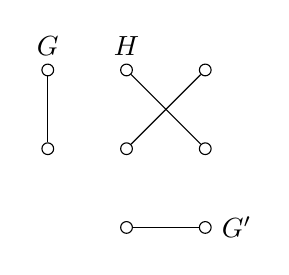
\begin{tikzpicture}[n/.style = {draw, circle, inner sep=1.5pt}]
			\node[n] at (0,1) (1) {};
			\node at (0,2.3) {$G$};
			\node[n] at (0,2) (2) {};
			\node[n] at (1,0) (3) {};
			\node[n] at (2,0) (4) {};
			\node at (2.4,0) {$G'$};
			\draw (1) -- (2);
			\draw (3) -- (4);
			\node[n] at (1,1) (5) {};
			\node[n] at (1,2) (6) {};
			\node[n] at (2,1) (7) {};
			\node[n] at (2,2) (8) {};
			\node at (1,2.3) {$H$};
			\draw (5) -- (8);
			\draw (6) -- (7);
		\end{tikzpicture}
		\caption{Simple example of graph product, where both $G$ and $G'$ are $P_1$.}
	\end{figure}
	
	\begin{defn}[Graph dimension]
		For a graph $G = (V,E)$ we define dimension $\dim(G) = \min(|I|)$ and $G$ is induced subgraph of $\prod_{i \in I} K_{n(i)}$.
	\end{defn}
	
	\begin{thm}
		For every $G$ there exists $n(i); i \in I$ such that $G$ is induced subgraph of $\prod_{i \in I} K_{n(i)}$.
	\end{thm}
	
	\begin{example}
		Lets see some examples of dimensions of graphs, where some may be easier and some harder. Firstly trivially $\dim(K_n) = 1$. Secondly for graph $G$ consisting of a isolated vertex and $K_n$ we have that $\dim(G) = n$. Lastly for a graph $H$ of a matching we get that $\dim(H) = \log n$ which was proved by Lovász, Pultr and Nešetřil.
	\end{example}
	
	When we take a graph $G_{V,1/2}$ which is a random graph with $V$ vertices and every edge has probability $1/2$ that it exists. The lower bound $\dim(G_{V,1/2}) \geq \frac{n}{\log n}$ can be seen by a probabilistic argument and the fact that $\dim(G)$ corresponds to the covering of edges of complement of $G$ by equivalences. Moreover Guo and Warke showed that for constants $c,c'$ we have the following.
	
	$$
	c \frac{n}{\log n} \leq \dim(G_{V,1/2}) \leq c' \frac{n}{\log n}
	$$
\end{topic}

\begin{topic}{Back to STS}
	For STS $(v,3,1,2)$ simple hypergraph $(X, \M)$ where $\M$ contains on $k$ points at least $k-3$ triples; that is for $k \geq 4$. Erd\H os stated if there exists STS $(X, \M)$ such that on any $l$ points there are $\leq l-3$ edges. This was proven as being true.
\end{topic}

\begin{topic}{Large BIBD}
	But what about $|\M| \geq n^{1 + \epsilon}$? This will be shown as being actually hard. We will talk about it more later.
\end{topic}